% Klassenarbeit Mathe 9b 18.5.2017
\documentclass [ngerman,12pt]{exam}
\usepackage[a4paper, total={16cm, 26cm}]{geometry}
\usepackage{amsfonts}
\usepackage{amsmath}
\usepackage{ngerman}
\usepackage{gensymb}
\usepackage[utf8]{inputenc}
\usepackage{tabularx}
\usepackage{tikz}
\usepackage{tkz-euclide}
\usetkzobj{all}
\usetikzlibrary{calc}
\usepackage{pgfplots}
\pgfplotsset{
  compat=1.12,
  axis lines=middle
}

\pointpoints{Punkt}{Punkte}
\bonuspointpoints{Bonuspunkt}{Bonuspunkte}
\renewcommand{\solutiontitle}{\noindent\textbf{Lösung:}%
\enspace}

\runningfooter{Klasse 9b}{Klassenarbeit Mathematik, 18.5.2017}{Seite \thepage\ von \numpages}
\runningfootrule

\chqword{Frage}
\chpgword{Seite}
\chpword{Punkte}
\chbpword{Bonus Punkte}
\chsword{Erreicht}
\chtword{Gesamt}

\hpword{Punkte:} % Punktetabelle
\hsword{Ergebnis:}
\hqword{Aufgabe:}
\htword{Summe}

\begin{document}
\noindent {\bf Name}:\\
\noindent {\bf Vorname}:\\
\hrule

\begin{center}
{\large\bf Klassenarbeit zu quadratischen Funktionen und Gleichungen}\\[2mm]
Hilfsmittel: Geodreick und Taschenrechner\\
Gymnasium Tiergarten\hfill 18. Mai 2017\\
Klasse 9b, Mathematik\hfill Bearbeitungszeit: 75 Minuten

\addpoints\gradetable[h][questions] 
\end{center}
\hrule
\medskip

%%%%%%%%%%%%%%%%%%%%%%%%%%%%%%%%%%%%
\begin{questions}

\question \textbf{Verschieben, Spiegeln und Strecken}
\begin{parts}
\part Gib jeweils Funktionsgleichungen für die resultierenden Funktionen an.
\begin{subparts}
\subpart[1] Die Normalparabel wird um den Faktor *A*drei***zwei*B* gestreckt und dann um *A*zwei nach oben***drei nach links*B* verschoben.
\par\medskip
$f(x)=$
\par\medskip
\subpart[1] Die Normalparabel wird an der X-Achse gespiegelt und dann um *A*drei nach rechts***zwei nach unten*B* verschoben.
\par\medskip
$f(x)=$
\par\medskip
\subpart[1] Die Normalparabel wird mit dem Faktor *A*$\frac{2}{3}$***$\frac{1}{2}$*B* gestaucht und dann um *A*zwei nach unten***eins nach oben*B* verschoben.
\par\medskip
$f(x)=$
\par\medskip
\end{subparts}
\part[3] Markus behauptet: ``Wenn ich die Normalparabel um eine positive Zahl $e$ nach *A*oben***unten*B* verschiebe und dann an der X-Achse spiegele, erhalte ich dieselbe Funktion, wie wenn ich die Normalparabel zuerst an der X-Achse spiegele und dann um $e$ nach *A*unten***oben*B* verschiebe.'' Stimmst Du ihm zu? Begründe Deine Aussage.
\vspace{2cm}
\end{parts}

\question \textbf{Schreibweisen}. Wir haben verschiedene Schreibweisen für quadratische Funktionen kennengelernt. Gib für jede der folgenden Funktionen an, ob es sich um eine quadratische Funktion handelt, und falls ja, ob sie in \underline{Normalform}, in \underline{Scheitelpunktform}, in \underline{Nullstellenform} oder \underline{keiner} der drei Formen notiert ist.
\begin{parts}
\part[2] $f(x)=*A*x+x(x+1)***3x^2+x+1*B*$\vspace{0.7cm}
\part[2] $f(x)=*A*(x-1)(x+4)***(x+3)-(x+2)*B*$\vspace{0.7cm}
\part[2] $f(x)=*A*3(x+5)-3***3(x+5)^2-3*B*$\vspace{0.7cm}
\end{parts}

\pagebreak

\question \textbf{Scheitelpunkt und Scheitelpunktform}
\begin{parts}
\part Die Schreibweise $a(x-d)^2+e, a\neq0$ bezeichnet man als ``Scheitelpunktform'' einer quadratischen Funktion, da man die Koordinaten des Scheitelpunkts direkt aus der Funktionsgleichung ablesen kann. Welchen Scheitelpunkt haben jeweils die folgenden Funktionen?
\begin{subparts}
\subpart[1] $f(x)=*A*5(x-2)^2-3***3(x+1)^2+2*B*$\hspace{2cm}$S(~~~~~|~~~~~)$\\
\subpart[1] $f(x)=*A*-\frac{1}{2}x^2+4***\frac{2}{3}x^2+3*B*$\hspace{2cm}$S(~~~~~|~~~~~)$\\
\subpart[1] $f(x)=*A*(x+1)^2***(x-2)^2*B*$\hspace{2cm}$S(~~~~~|~~~~~)$\\
\end{subparts}
\part[4] Wandle $f(x)=*A*2x^2-2x-2***3x^2+3x-9*B*$ in Scheitelpunktform um.\vspace{7cm}
\part[2] Maggy hat die Funktion $f(x)=*A*4x^2+x+1***2x^2+4x+1*B*$ in Scheitelpunktform umgewandelt und $f'(x)=*A*4\left(x+\frac{1}{8}\right)^2+1***2(x+2)^2-3*B*$ als Ergebnis erhalten. Überprüfe, ob sie richtig gerechnet hat.
\vspace{3cm}
\end{parts}

\pagebreak

\question \textbf{Nullstellen}
\begin{parts}
\part Bestimme die Nullstelle(n) der folgenden Funktionen. Schreibe die Lösungsmenge auf.
\begin{subparts}
\subpart[3] $f(x)=*A*x^2+3+x^2***x-5x^2*B*$\vspace{5.5cm}
\subpart[3] $f(x)=*A*(x-2)\cdot5x***2x^2+3*B*$\vspace{5.5cm}
\subpart[3] $f(x)=*A*-x^2+4***(x-1)(x+2)*B*$\vspace{5.5cm}
\subpart[4] $f(x)=*A*2x+3x^2-1***x^2-3x^2+2*B*$\vspace{5.5cm}
\end{subparts}

\pagebreak

\part Gib für die folgenden Parabeln jeweils eine Funktionsgleichung an.
\begin{subparts}
\subpart[2] eine nach oben geöffnete Parabel mit *A*den Nullstellen 3 und 4***einer doppelten Nullstelle bei 2*B*
\par\medskip
$f(x)=$
\par\medskip
\subpart[2] eine nach unten geöffnete Parabel mit *A*einer doppelten Nullstelle bei -7***den Nullstellen 0 und 4*B*
\par\medskip
$f(x)=$
\par\medskip
\subpart[2] eine Parabel mit Streckfaktor *A*5 und Nullstellen bei -2 und 2***2 und Nullstellen bei 3 und 4*B*
\par\medskip
$f(x)=$
\par\medskip
\end{subparts}
\part[2] Gib das Beispiel einer quadratischen Funktion an, die sich nicht in Nullstellenform bringen lässt, und begründe, warum das mit Deinem Beispiel nicht möglich ist.
\vspace{3cm}
\end{parts}
\question \textbf{Weiterführende Aufgabe}
\begin{parts}
\part[4] Zeichne die Funktionen *A*$f(x)=x^2$ und $g(x)=\frac{4}{3}x$***$f(x)=x^2$ und $g(x)=\frac{3}{2}x$*B* in das Koordinatensystem und lies die Schnittpunkte von $f$ und $g$ aus Deiner Zeichnung ab.
\begin{center}
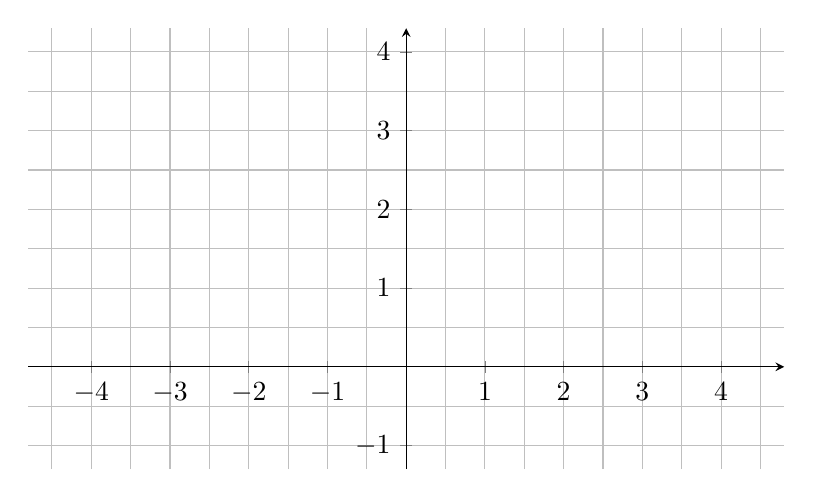
\begin{tikzpicture}
  \begin{axis}[
    xmin=-4.8,xmax=4.8,
    ymin=-1.3,ymax=4.3,
    x=1cm,
    y=1cm,
    minor tick num=1,
    minor tick length=0pt,
    grid={both}
    ]
  \end{axis}
\end{tikzpicture}
\end{center}
\part[4] Bestimme die Schnittpunkte von $f$ und $g$ rechnerisch, indem Du die beiden Funktionsterme gleichsetzt. Hinweis: Wenn Du beide Terme auf die linke Seite des Gleichheitszeichens bringst, erhältst Du eine quadratische Gleichung und kannst so die $x$-Werte der Schnittpunkte bestimmen.
\end{parts}

\end{questions}
\end{document}
